\documentclass{article}

\usepackage{../preamble}
\standalonetrue

\pagestyle{fancy}
\fancyhf{}
\rhead{Section \thesection}
\lhead{PHYS 304 Lecture 22}
\rfoot{Page \thepage}


\title{PHYS 304 Lecture 22}
\author{Ashtan Mistal}
\date{!!!}

\begin{document}

\ifstandalone
\maketitle
\fi

\graphicspath{{./Lecture22/}}


\section{Review of key points form last lecture}

% copy from slides

\section{Today}

\begin{itemize}
    \item Derive the spectrum of allowed eigen values of the shared eigen state of the $\hat{L}^2$ and the $\hat{L}_z$ operators using only the properties of the $\hat{L}_\pm$ operators and some basic physics.
    \item Derive the associated shared set of eigen functions. 
    
    \item Hopefully start a discussion of spin.

\end{itemize}

 \subsection{General spectrum of common eigenstates of the $\hat{L}^2$ and $\hat{L}_z$ operators}
 
 Use the raising and lowering operators to derive the spectrum of eigen values of the  $\hat{L}^2$ and $\hat{L}_z$ operators.  Roughly the same strategy as used in the ladder operator derivation of the eigen spectrum of the 1D Harmonic oscillator.


\begin{itemize}
    \item  Step 1: Define terms

\item Step 2: Show that the states $\hat{L}_\pm \ket{L_\lambda}$ are also eigen states of $\hat{L}^2$  with the same eigen value $\lambda$.

\item Step 3: Knowing that there must be a shared set of eigen functions with $\hat{L}_z$, what are the corresponding eigen values?

\item Step 4: Introduce some basic physics (any component can’t be larger than the total angular momentum) 

\item Step 5: Implications (there must be a maximum eigen value of the $\hat{L}_z$ operator 

\item Step 6: Apply same strategy to find the lowest possible (negative) eigen value of the $\hat{L}_z$ operator consistent with $|\mu|^2 \leq \lambda$  

\item Step 7: The full spectrum.
\end{itemize}





 
 Spectrum of the total angular momentum and $L_z$ component in a common basis. 
 
 Recall: $[\hat{L}, \hat{L}_\pm] = 0$, and $[\hat{L}_z, \hat{L}_\pm] = \pm \hbar \hat{L}_\pm$
 
 - Assume we have eigen functions of $|\hat{\vec{L}}^2|  \hat{L}^2$, then $\hat{L}^2 = \ket{\psi_\lambda} = \lambda \ket{\psi_\lambda}$, what can we say about $\hat{L}_\pm \ket{\psi_\lambda}$?
 
 $$\hat{L}^2 (\hat{L}_\pm \ket{L_\lambda}) = \hat{L}_\pm \hat{L}^2 \ket{\psi_\lambda} (commute) = \lambda \left( \hat{L}_\pm \ket{L_\lambda} \right)$$
 
 Therefore, $ \hat{L}_\pm \ket{L_\lambda}$ is also an eigen function of $\hat{L}^2$ with the same eigen value. 
 
 Let's look at $\hat{L}_z \left( \hat{L}_\pm \ket{\psi_\pm} \right) = \hat{L}_z \left( \hat{L}_x \pm i \hat{L}_y \right) \ket{\psi_\lambda}$
 
 Assume  $\ket{\psi_\lambda}$ is an eigen function of $\hat{L}^2$, and $\hat{L}_z$ with eigen value $\mu$ of $\hat{L}_z$. 
 
 $$\Rightarrow \hat{L}_z \ket{\psi_{\lambda, \mu}} = \mu \ket{\psi_{\lambda, \mu}}$$
 
 Using $[\hat{L}_z, \hat{L}_y] = i\hbar \hat{L}_x$ and $[\hat{L}_z, \hat{L}_y] = i \hbar \hat{L}_y$
 
 $$\hat{L}_z \hat{L}_x = i \hbar L_y + \hat{L}_x \hat{L}_z$$
 
 $$\hat{L}_z \hat{L}_y = -i \hbar \hat{L}_x + \hat{L}_y \hat{L}_z$$
 
 $$\rightarrow \hat{L}_z \left( \hat{L}_\pm \ket{\psi_{\lambda, \mu}} \right) = \left( \left( i \hbar \hat{L}_y + \hat{L}_x \hat{L}_z \right) \pm i \left( \hat{L}_y \hat{L}_z - i \hbar \hat{L}_x \right) \right) \ket{\psi_{\lambda, \mu}}$$
 
 $$ = \left( i \hbar  \hat{L}_y \pm \hbar \hat{L}_x \right) \ket{\psi_{\lambda, \mu}} + \mu \left( \hat{L}_\pm \ket{\psi_{\lambda, \mu}} \right)$$
 
 $$\hat{L}_z \left( \hat{L}_\pm \ket{\psi_{\lambda, \mu}} \right) = \left( \pm \hbar + \mu \right) \hat{L}_\pm \ket{\psi_{\lambda, \mu}} \Rightarrow $$
 
 $\left( \pm \hbar + N \right)$ is the eigen value of the new eigen function of $\hat{L}_z = \hat{L}_\pm \ket{\psi_{\lambda, \mu}}$
 
 $\hat{L}_+$ operating on a common eigen function of $\hat{L}^2$ and $\hat{L}_z$ produces another common eigen function with the same eigen value of $\hat{L}^2$ ($\lambda$), but the eigen value of $\hat{L}_z$ is the original state's eigen value ($\mu$) $\pm \hbar$. 
 
 Now add physics:
 
 $$\braket{\hat{L}_z} \leq \braket{\hat{L}^2}$$
 
Therefore $\braket{\hat{L}^2}$ must be a max value of $N$ and associated by "top" eigen function $\ket{\psi^t_{\lambda, \mu}}$ such that $\hat{L}_+ \ket{\psi^t_{\lambda, \mu}} = 0$

Let $\hat{L}_z \ket{\psi^t_{\lambda, \mu_t}} = \hbar \ell \ket{\psi^t_{\lambda, \mu_t}}$

$\mu_t = \hbar \ell$, and we know that $\hat{L}^2 \ket{\psi^t_{\lambda, \mu_t}} = \lambda \ket{\psi^t_{\lambda, \mu_t}}$
 
 
To proceed, expand $\hat{L}^2$ in terms of $\hat{L}_\pm$ and $\hat{L}_z$

$$\hat{L}^2 = \hat{L}_x^2 + \hat{L}_y^2 + \hat{L}_z^2 = \hat{L}_- \hat{L}_+ + \hat{L}_z^2 + \hat{O}$$

$$\hat{L}_- \hat{L}_+ = \left( \hat{L}_x - i \hat{L}_y \right) \left( \hat{L}_x + \hat{L}_y \right) = \hat{L}^2_x + \hat{L}_y^2 + i [\hat{L}_x, \hat{L}_y] = \hat{L}_x^2 + \hat{L}_y^2 - \hbar \hat{L}_z$$

$$\hat{L}^2 = \hat{L}_- \hat{L}_+ + \hat{L}_z^2 + \hbar \hat{L}_z^2 \Rightarrow \hat{L}^2 \ket{\psi^t_{\lambda, \mu_t}} = (O + \left( \hbar \ell \right)^2 + \hbar \hbar \ell)\ket{\psi^t_{\lambda, \mu_t}}  = \hbar^2 \ell (\ell + 1)\ket{\psi^t_{\lambda, \mu_t}} = \lambda \ket{\psi^t_{\lambda, \mu_t}}$$

Same analysis on "bottom" most eigen state of $\hat{L}_a \Rightarrow \lambda = \hbar^2 \tilde{\ell}(\tilde{\ell} - 1) \Rightarrow \tilde{\ell} = -\ell \Rightarrow \lambda = \hbar^2 \ell(\ell + 1)$

(Other option, $\tilde{\ell} = \ell + 1$, would mean the lower state has a higher value than the top)

So conclude that shared eigen functions of $\hat{L}^2$ and $\hat{L}_z$ have common $\hat{L}^2$ eigen value of $\lambda = \hbar^2 \ell(\ell + 1)$, and $\hat{L}_z$ has a set of eigen values $\mu + n \hbar$. But, also know that integer number must connect lowest and highest $\Rightarrow$

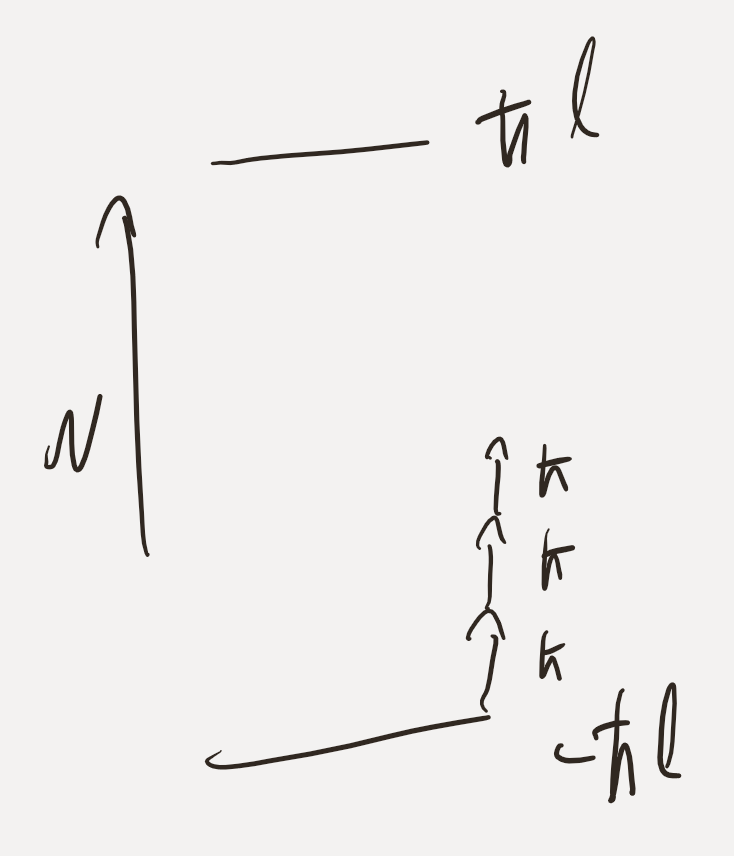
\includegraphics[width = 0.2 \textwidth]{Lecture22/2.png}

(where N is increasing upwards)



$$\ell = \frac{N}{2}$$

where $N$ is an integer. 

$$- \hbar \ell \leq \mu \leq \hbar \ell$$

We now have very specific allowed values of $\lambda$ \textbf{and} the $\hat{L}_z$ eigen values. 

$\Rightarrow$ $\ell$ must be a $\frac{1}{2}$ integer or a full integer. So the allowed eigen values of $\hat{L}_z$ are:

$$-\hbar, \ell - \hbar(\ell-1),........\hbar(\ell - 1), ....... 2 \ell + 1$$

All associated with $\hat{L}^2$ eigen value of $\hbar^2 \ell(\ell + 1)$

$\ell$ must be half or full integer. 

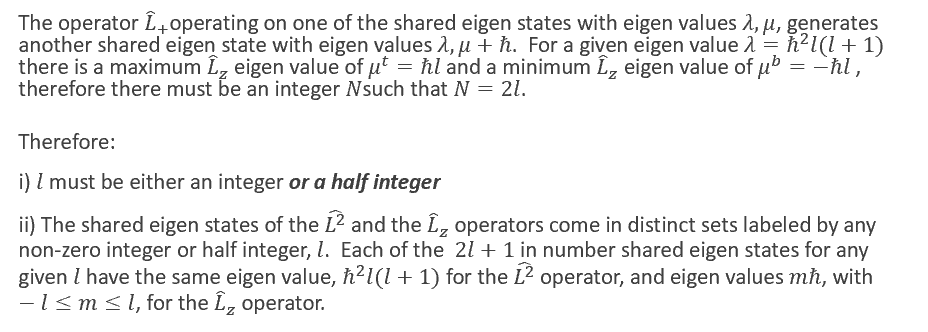
\includegraphics[width = 0.8 \textwidth]{Lecture22/3.png}

\section{The eigen functions}

Render  $\hat{L}^2$ and the $\hat{L}_z$ operators in the position basis (QM Hilbert space basis), then choose the spherical coordinate system to express the operators in terms of  $\theta, \phi, \hat{\theta}, \hat{\phi}$. (see text for derivation)   

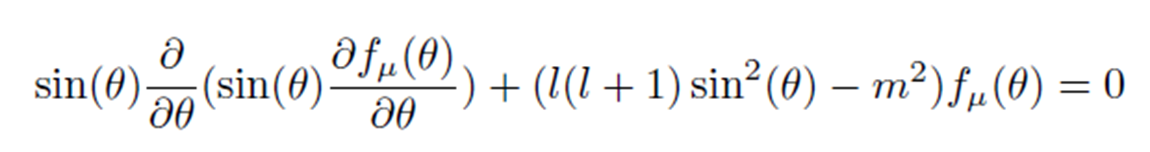
\includegraphics[width = 0.45 \textwidth]{Lecture22/4.png}


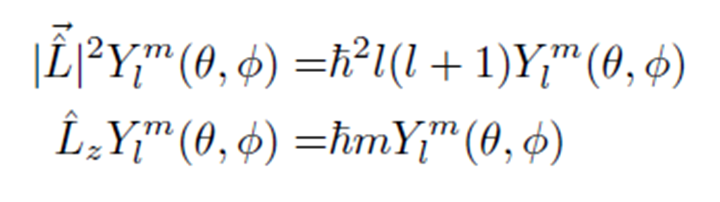
\includegraphics[width = 0.3 \textwidth]{Lecture22/5.png}

Eigenfunctions?

Get $\hat{L}_x, \hat{L}_y, \hat{L}_z, \hat{L}^2$ in spherical coordinates and solve $\hat{L}_{z, \vec r} \psi_{Lz}(\theta,\phi) = \mu \psi_{L,z} (\theta, \phi)$, and  $\hat{L}_r^2 \psi_{L,z} (\theta,\phi) = \lambda \psi_{L,z} (\theta, \phi)$

$$L_{z,\vec{r}} = - i \hbar \frac{\partial}{\partial \phi}, \hat{L}^2 = - \hbar^2 \left( \frac{1}{\sin{\theta}} \frac{\partial}{\partial \theta} \left( \sin(\theta) \frac{\partial}{\partial \theta} \right) + \frac{1}{\sin^2 \theta} \frac{\partial^2}{\partial \phi^2} \right)$$

% copy example




\end{document}